

Turbomachines are part of a more general class of machines, that
exchange energy between the fluid traversing it and mechanical energy
supplied to or extracted from the machine. The useful energy of a
working fluid is at rest stored as (excess) pressure; when the fluid
is in motion, its energy is also partly kinetic. Both forms of energy
can be converted into the other.
\begin{figure}[!h]
  \centering
  \begin{subfigure}{0.49\textwidth}
    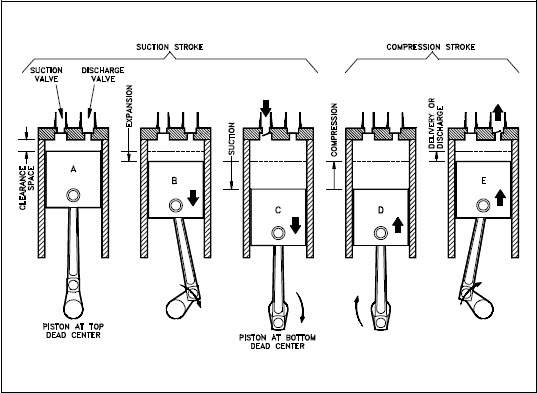
\includegraphics[width=\textwidth]{introduction/pistonCompressor.png}
    \caption{Singly acting piston compressor}
  \end{subfigure}
  \begin{subfigure}{0.49\textwidth}
    \hfill
    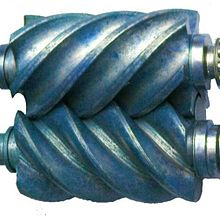
\includegraphics[width=0.8\textwidth]{introduction/LysholmScrewCompressor.png}
    \caption{Screw compressor (Wikimedia Commons)}
  \end{subfigure}
  \caption{Volumetric compressors}
  \label{fig:volumetricCompressors}
\end{figure}
Volumetric machines will transfer energy through pressure work during
compression or expansion of a temporarily closed volume, without any
(significant) contribution of kinetic energy. Figure
\ref{fig:volumetricCompressors} illustrates this through two
representative examples. The piston compressor ingests a certain
volume of air, closes the cylinder, then compressers the volume before
finally discharging the air to the outlet. The Lysholm screw rotors
form a progressing cavity of constant volume moving from left to
right. The enclosed air is then compressed from the inlet to the
outlet pressure. 
\begin{figure}[!h]
  \centering
  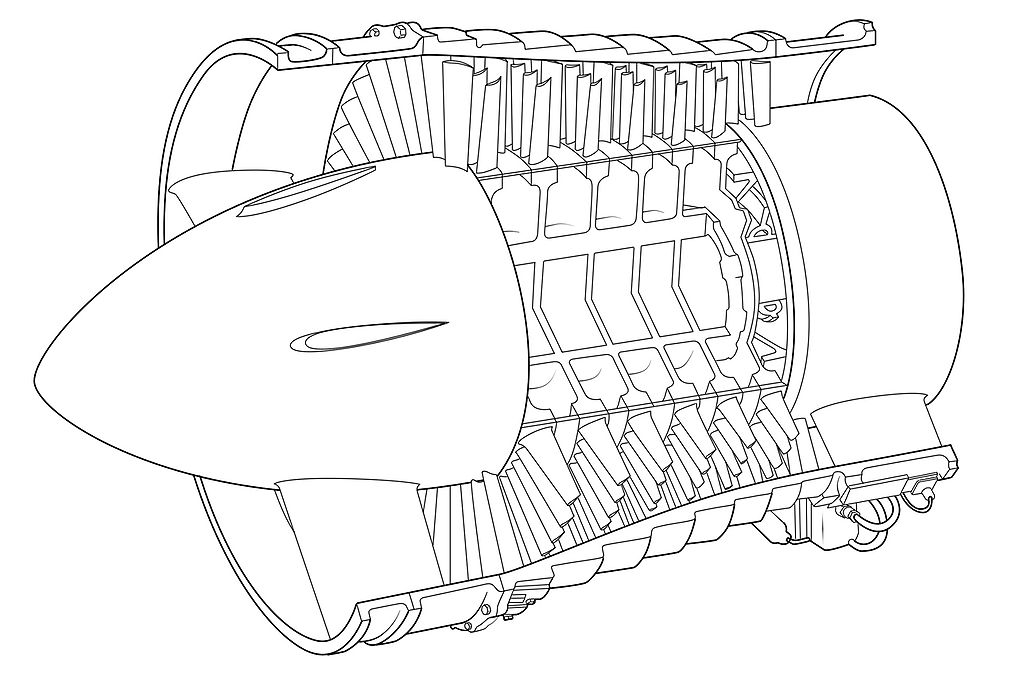
\includegraphics[width=0.8\textwidth]{introduction/LPCompressorOlympusB01TurboJet.png}
  \caption{6-stage compressor of the Olympus BOI.1 Turbojet (Wikimedia
    Commons)}
  \label{fig:turbocompressor}
\end{figure}

In contrast, turbomachines do not confine the working fluid in a
closed volume, but are fully open: fluid can freely pass from inlet to
outlet. The energy exchange then happens due to dynamic effects during
the motion of the fluid; therefore energy is exchanged through the
intermediary of kinetic energy.  As an example, the turbojet
compressor in figure \ref{fig:turbocompressor} pushes the flow from
the front to the back of the machine via lift forces on rotating and
stationary rows of equispaced airfoils or \emph{blades}.  Obviously
the energy can only be transferred by rotating blade rows or
\emph{rotors} whereas stationary blade rows or \emph{stators} are used
to condition the flow before or after a rotor. A compressor/pump
stator is typically positioned downstream the rotor, and used to
convert the excess kinetic energy imparted by the upstream rotor into
pressure. In turbines, the stator is positioned upstream to convert
pressure into a high level of kinetic energy for power extraction in
the downstream rotor. Due to this different roles, rotors and stators
are conceptually grouped in pairs, called \emph{stages}.

Turbomachines can be classified following a number of criteria:
\begin{itemize}
\item according to the direction of the energy exchange
  \begin{itemize}
  \item \emph{turbines} convert energy contained in the fluid to
    mechanical energy at the shaft;
  \item \emph{compressors}, \emph{ventilators} or \emph{pumps}
    increase the energy of the fluid.
  \end{itemize}
\item according to the working fluid, distinguishing between
  \emph{hydraulic} machines and those working with compressible media
  such as gas or steam;
\item according to the flow direction with respect to the axis, as
  illustrated in figure \ref{fig:axialVsRadial}:
  \begin{itemize}
  \item in \emph{axial} machines, the motion of the fluid follows the
    axis of the machine. 
  \item in \emph{radial} machines, the flow is mainly directed
    radially in- or outward;
  \item in \emph{mixed flow} machines, the main flow path is neither
    purely axial nor radial. 
  \end{itemize}
\end{itemize}
\begin{figure}[!h]
  \centering{
    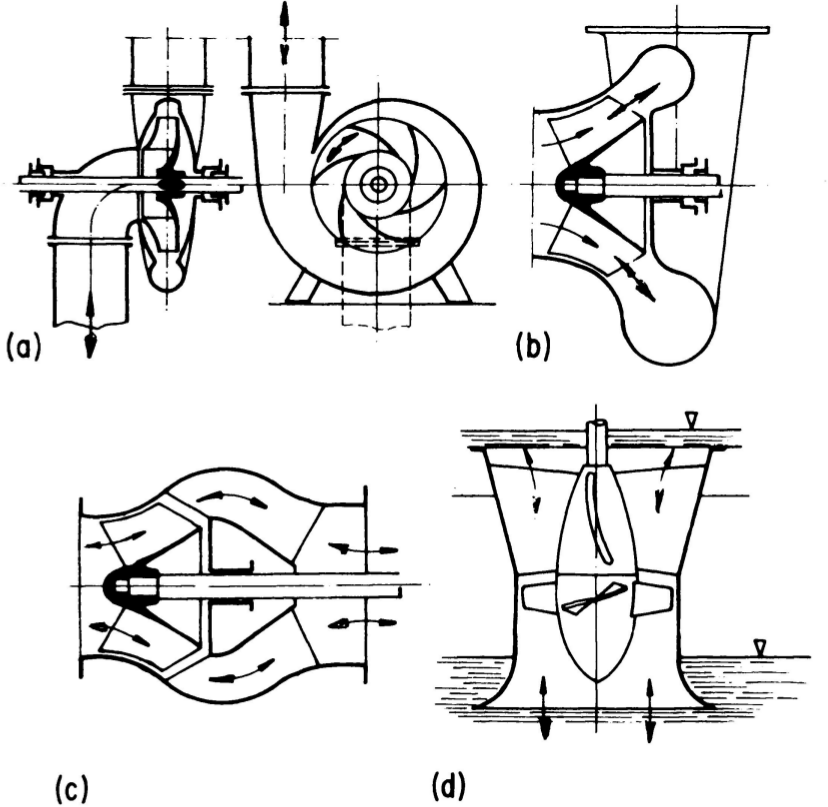
\includegraphics[width=0.8\textwidth]{introduction/axialVsRadial.png}
  }
  \caption{Classification (of pumps) following direction: radial (a),
    mixed (b-c) and axial (d).}
  \label{fig:axialVsRadial}
\end{figure}

% \begin{figure}[!h]
%   \centering{
%     \begin{subfigure}{0.8\textwidth}
%       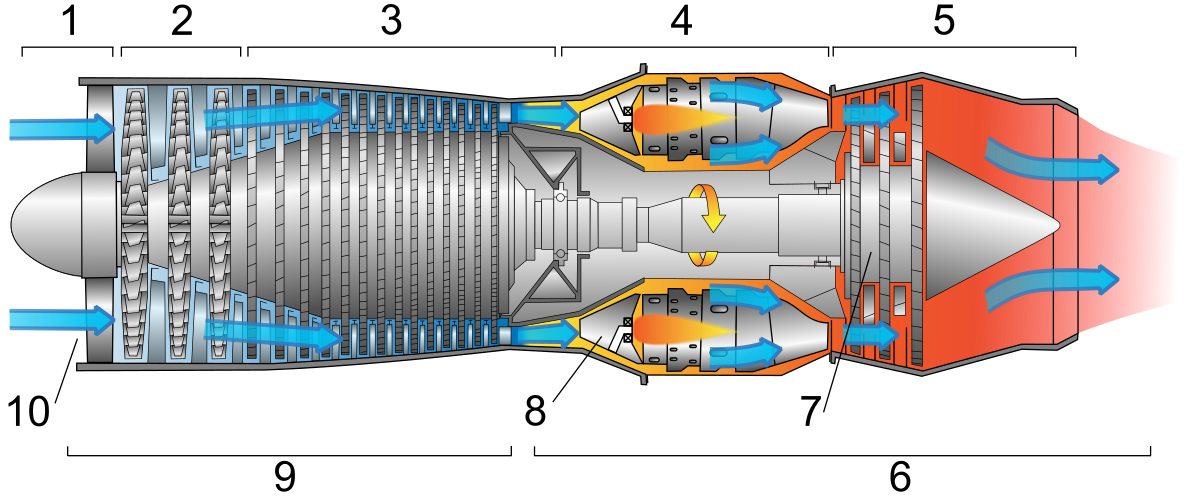
\includegraphics[width=\textwidth]{introduction/jetEngine.png}
%       \caption{Multistage axial turbomachinery components in a
%         military jet engine: 3-stage low pressure (LP) compressor (2);
%         14-stage high pressure (HP) compressor (3); 2-stage HP turbine
%         and single stage LP turbine (7). Image from Wikimedia Commons
%         \cite{wikimedia_jetEngine}.}
%     \end{subfigure}
%   }
%   \centering{
%     \begin{subfigure}{0.7\textwidth}
%       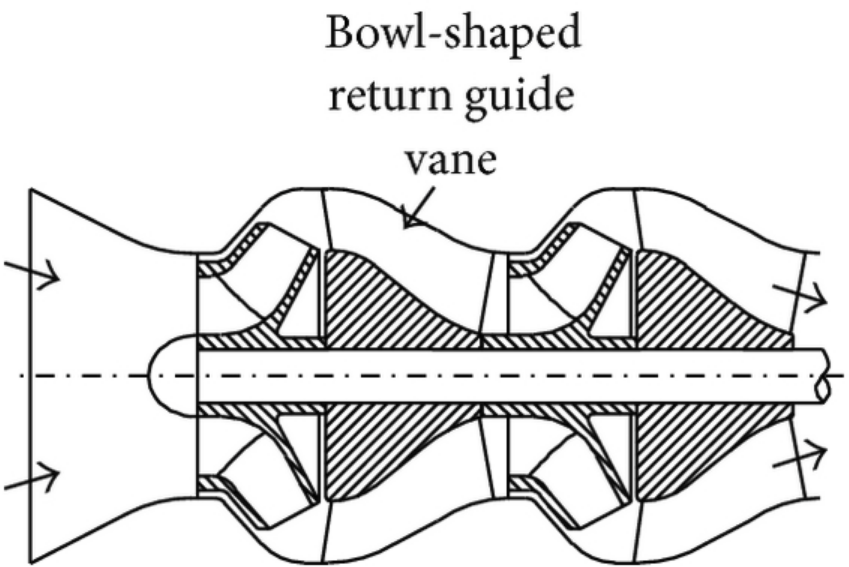
\includegraphics[width=\textwidth]{introduction/bowlPump.png}
%       \caption{Multistage mixed flow (``bowl'') pump. From Zhang
%         \etal \cite{ZSX+13}.}
%     \end{subfigure}
%   }
%   \caption{Examples of multistage turbomachinery components}
%   \label{fig:multistage}
% \end{figure}

\section{Organisation of the course}

The course is organized as follows. In the first chapter we will
recapitulate and introduce some general principles from fluid
mechanics. This involves the introduction to the notation used
throughout the text, the derivation and (energetic) interpretation of
the Navier-Stokes equations of fluid motion. The second chapter will
introduce specific subjects related to turbomachinery specialisations
of these equations to turbomachinery flows.

The subsequent chapters are dedicated to the different types of
turbomachines, discussing flow, performance and operation. The
chapters are organized following the matrix in table
\ref{tab:organisation}.
\begin{table}[!h]
\centering{
\begin{tabular}{c|cc}
  & {\bf energy addition}
  & {\bf energy extraction} \\
  \hline
  {\bf incompressible flow} 
  & pumps, ventilators %  (chap. \ref{chap:pumps} ) 
  & hydraulic turbines % (chap. \ref{chap:hydraulicTurbines}) 
  \\
  & & wind turbines \\ %  (chap. \ref{chap:windTurbines} ) \\
  \hline
  {\bf compressible flow} 
  & compressors %  (chap. \ref{chap:compressors}) 
  & turbines % (chap. \ref{chap:turbines}) 
  \\
  %& propellers (chap. \ref{chap:propellors}) & \\
\end{tabular}}
\caption{Organisation of chapters dedicated to turbomachinery components.}
\label{tab:organisation}
\end{table}
A few additional chapters are introduce the fundamental phenomena
occurring in the incompressible or compressible flow regimes, before
entering the chapters dedicated to specific machinery components. A
first chapter will discuss incompressible flows and hydraulic circuits
and cavitation, whereas a second chapter discusses compressible flow
thermodynamics and sonic effects.

\section{Acknowledgments}

These course notes are adapted from the notes of Prof. L{\'e}onard (ULg) and borrowed additional material from several sources, including the books by Prof. Dick \cite{EDick} and Dr. Vavra \cite{Vavra}, Dr. Franc \etal \cite{LaCavitation} and Dr. Stepanoff \cite{Stepanoff}.


%%% Local Variables: 
%%% mode: latex
%%% TeX-master: t
%%% End: 
